\section{Project specifications}
\label{sec:project_specifications}

For the project, you are free to choose one of the following two projects. You are also free to propose your own project (with the elements you have in the lab kit, or with other if you have some additional elements at home). In that case, please contact the teaching staff so that we can agree on the specifications of your self-proposed project. 

\subsection{Distress beacon specifications}

The aim of this project is to build an emergency beacon that is capable of sending three types of distress signals, as shown in Figure~\ref{fig:distress_beacon}: 
\begin{enumerate}
	\item a luminous signal sending morse code; 
	\item an audio signal sending morse code; 
	\item a visual flag type signal sending semaphore code. 
\end{enumerate}
Morse code is a succession of short and long luminous or audio signals, which can describe the letters of the alphabet. Semaphore code uses two flags to describe the different letters of the alphabet: \url{https://gregheo.com/images/blog/semaphore-alphabet.jpg} (note that your servos can only rotate $180^{\circ}$, so not all letters can be done. You are free to change the combination of flags for those letters). Different inputs will be used to allow different functionalities of the distress beacon. 

\begin{figure}[h]
	\centering
	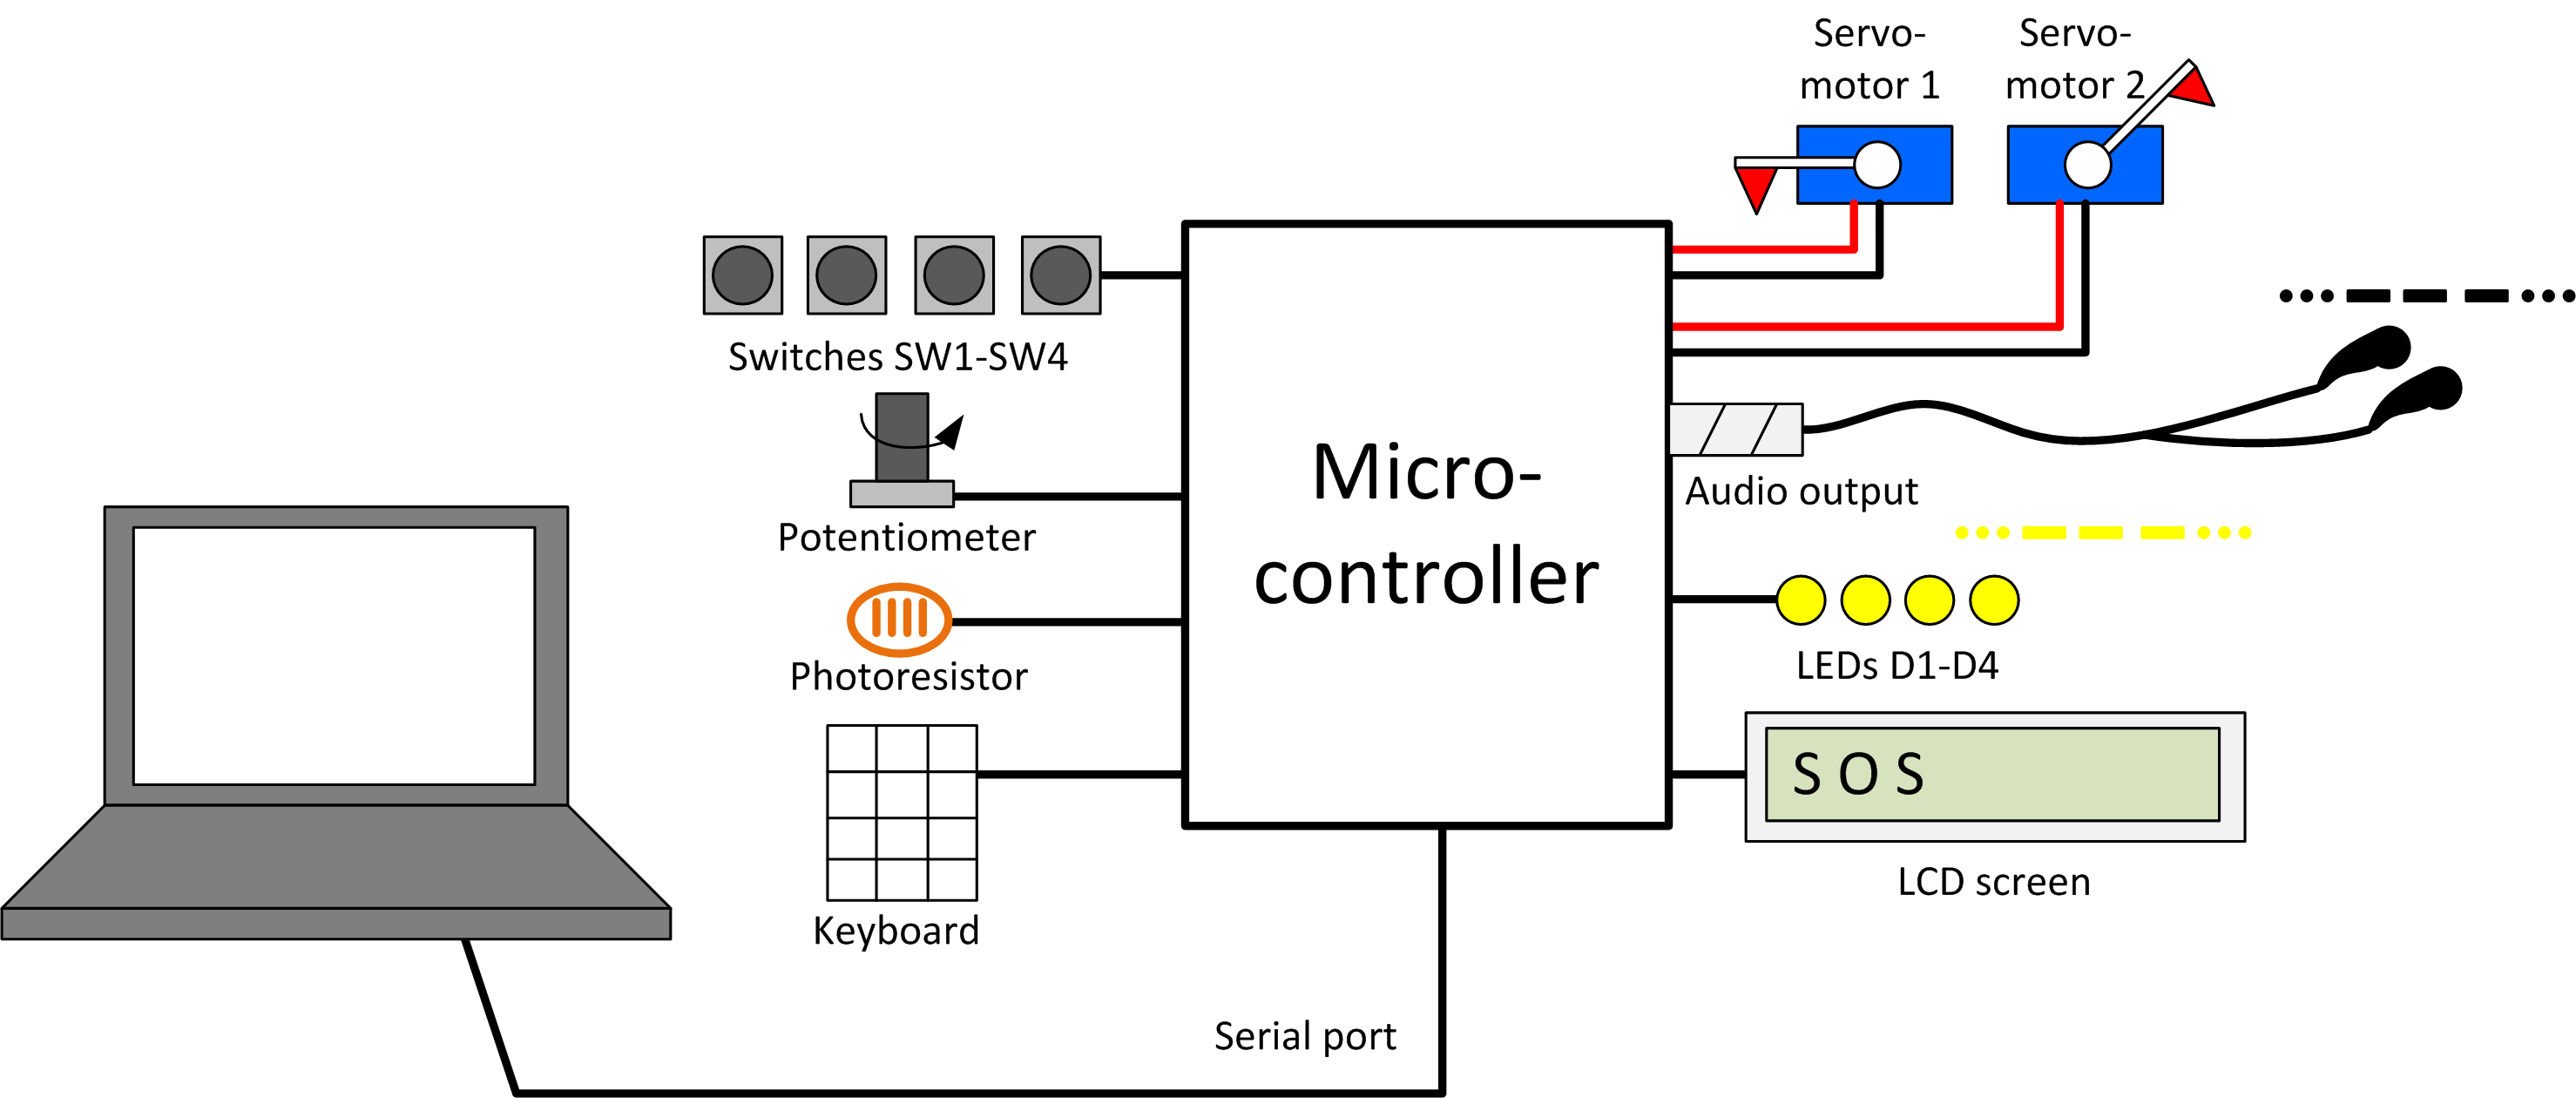
\includegraphics[width=5in]{distress_beacon.png}
	\caption{Schematic representation of the distress beacon inputs and outputs. }
	\label{fig:distress_beacon}
\end{figure}

The inputs should be configured as follows. 
\begin{itemize}
	\item \textbf{SW1:} When pressing switch SW1, the LEDs should light up and the audio output should emit a sound as long as the switch is pressed. When the switch is unpressed, the LEDs should go out and the audio output should stop emitting a sound. 
	\item \textbf{SW2:} When pressing switch SW2, the LEDs and audio output should emit a short morse signal. The short morse signal should be 250~ms long. 
	\item \textbf{SW3: } When pressing switch SW3, the LEDs and audio output should emit a long morse signal. The long morse signal should be 750~ms long. 
	\item \textbf{SW4 and Pot: } When turning the potentiometer (Pot), the flag should be going up according to the turning of the potentiometer. When pressing SW4, we change the flag that is controlled with the potentiometer. 
	\item \textbf{Photoresistor: } The photoresistor can detect whether there is ambient light or not. When there is light, only the audio output and semaphore flags should be active. When there is no light, only the audio output and the LEDs should be active. 
	\item \textbf{Keyboard: } We can use the keyboard to send a series of pre-recorded message. For example, pressing ``1'' and ``*'' should start sending ``SOS'' in morse and semaphore code. Pressing ``2'' and ``*'' should send ``BEAMS'' in morse and semaphore code. Other messages are for you to chose. 
	\item \textbf{Serial port: } The user computer can send ASCII characters through the serial port, which are then sent in morse and semaphore code by the distress beacon. The microcontroller also sends two types of characters to the user computer over the serial ports: ``.'' and ``-'' (which represents short and long morse signals that are sent by the distress beacon). 
	\item \textbf{LCD screen: } The LCD prints the ASCII characters that are sent by the distress beacon (this feature can only be used when using the keyboard or the serial port). You can also chose to print additional information on the LCD screen. 
\end{itemize}




\subsection{Never-lose specifications}

The aim of this project is to build a system that can play Google Chrome's \textit{dino} game autonomously (without ever losing of course). You can play it by opening a Chrome browser and typing the following URL: \url{chrome://dino}. When you press the spacebar, the game will launch. Your \textit{Never-lose} system should: 
\begin{enumerate}
	\item use the photoresistors to detect incoming obstacles on the screen; 
	\item use the servomotors to press the spacebar and the ``down'' arrow. 
\end{enumerate}
You can attach the photoresistors to your screen with some duck tape, the servomotors should be taped to the keyboard or held down with some weights to ensure that they don't move when pressing the computer's keys. 

\begin{figure}[h]
	\centering
	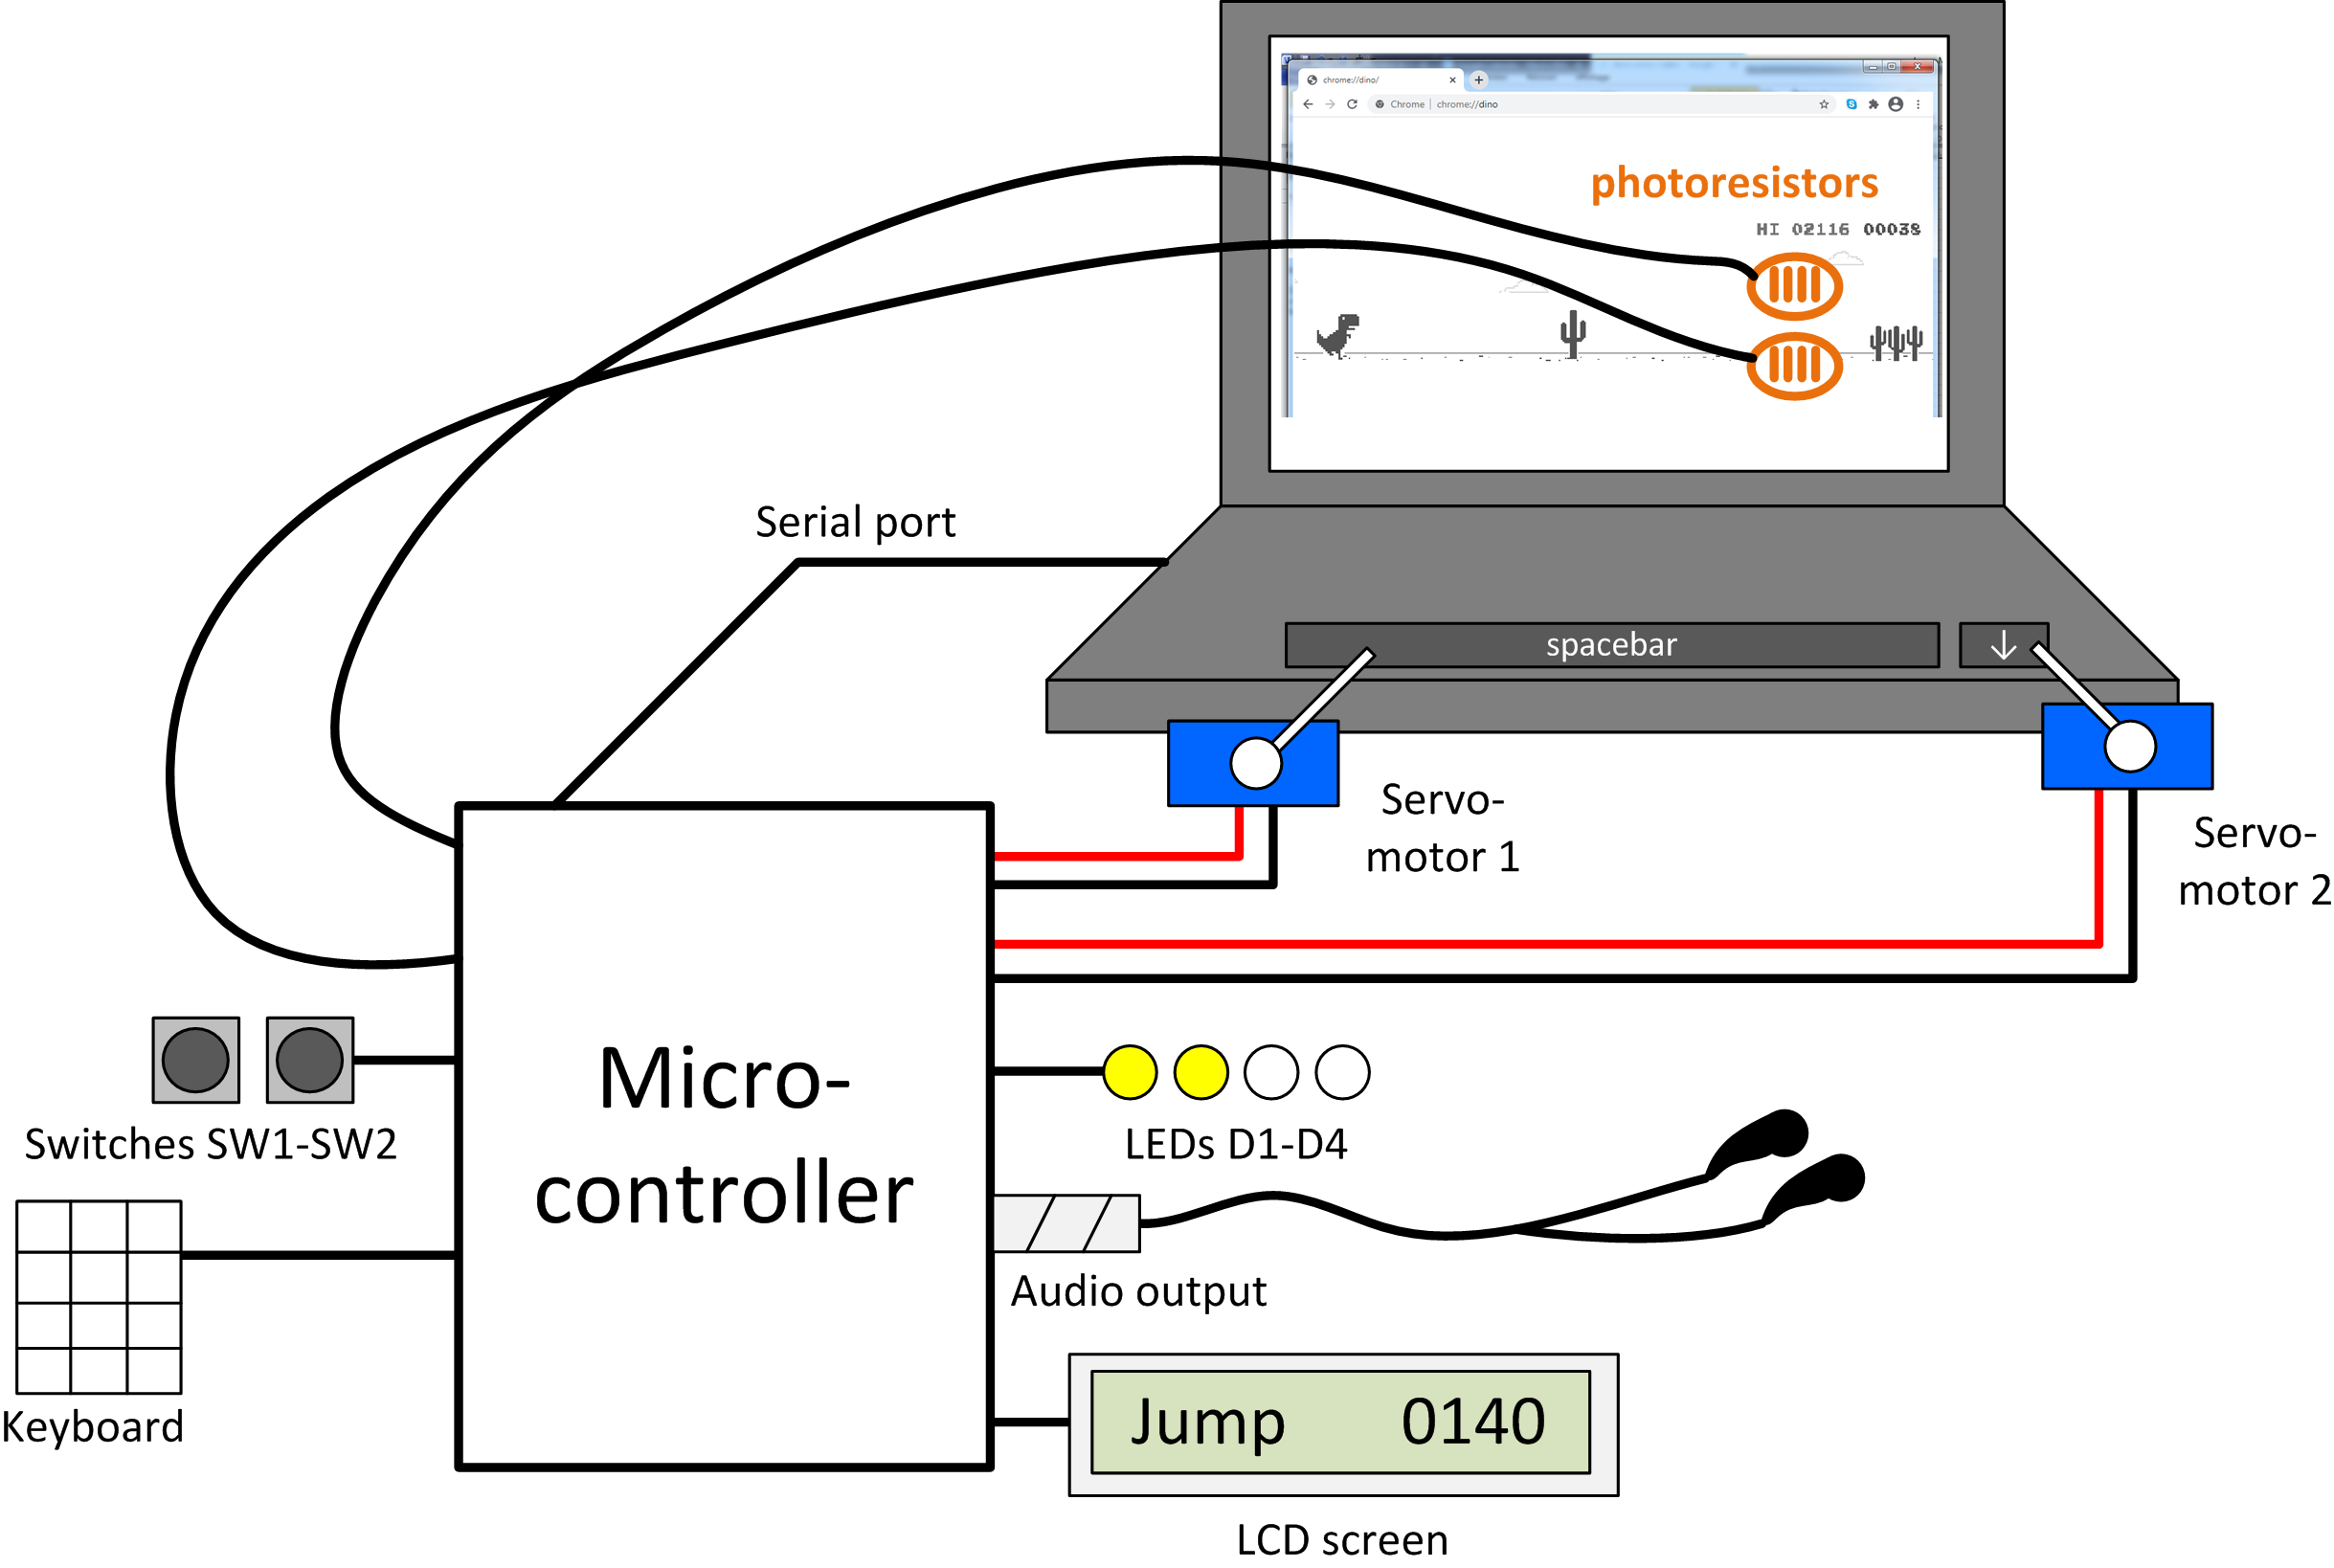
\includegraphics[width=5in]{never_lose.png}
	\caption{Schematic representation of the never-lose system. }
	\label{fig:never_lose}
\end{figure}

The inputs and outputs should be configured as follows. 
\begin{itemize}
	\item \textbf{SW1: } When pressing SW1, the servo controlling the spacebar should press the spacebar. 
	\item \textbf{SW2: } When pressing SW2, the servo controlling the down-arrow key should press the down-arrow key. 
	\item \textbf{SW3 and score counting: } When pressing SW3, the score should be reset to zero. The score should start increasing the first time the spacebar is pressed after resetting the score to zero (in the dino game, the score increases with 10 points per second). The score should be printed on the second half of the LCD. 
	\item \textbf{LED1-LED2: } These LEDs should light up when the dinosaur is jumping. 
	\item \textbf{LED3-LED4: } These LEDs should light up when the dinosaur is ducking. 
	\item \textbf{Photoresistor: } The photoresistors should be used to detect incoming obstacles (one photoresistor for the ground obstacles, one for the flying obstacles). 
	\item \textbf{Keyboard: } You can pick two keys of the microcontroller keyboard that should have the same effects as SW1 and SW2. 
	\item \textbf{Serial port: } The user computer can send the ``jump'' and ``duck'' command through the serial port (for example for launching the game), which should result in the correct servo pressing the correct key. The microcontroller should also send the following messages to the user computer over the serial ports: ``Jump'' and ``Duck'' when the dinosaur is jumping/ducking. 
	\item \textbf{LCD screen: } The LCD screen should print ``Jump'' when the dinosaur is jumping, ``Duck'' when the dinosaur is ducking. The second part of the LCD should print the score. 
	\item \textbf{Audio out: } The audio output should emit one sound when the dinosaur is jumping, another sound when the dinosaur is ducking. 
\end{itemize}

As a bonus, the following elements can be implemented: 
\begin{itemize}
	\item a system to detect when the day changes into night on the game; 
	\item ...
\end{itemize}









\subsection{Expected deliverables}

At the end of the project, we will expect the following deliverables: 
\begin{itemize}
	\item A fully-functional code that implements the project specifications; 
	\item A demo (or a video that you can take with your smartphone) of the prototype in action. 
\end{itemize}




